\documentclass[12pt,letterpaper]{article}
\usepackage{graphicx,textcomp}
\usepackage{natbib}
\usepackage{setspace}
\usepackage{fullpage}
\usepackage{color}
\usepackage[reqno]{amsmath}
\usepackage{amsthm}
\usepackage{fancyvrb}
\usepackage{amssymb,enumerate}
\usepackage[all]{xy}
\usepackage{endnotes}
\usepackage{lscape}
\newtheorem{com}{Comment}
\usepackage{float}
\usepackage{hyperref}
\newtheorem{lem} {Lemma}
\newtheorem{prop}{Proposition}
\newtheorem{thm}{Theorem}
\newtheorem{defn}{Definition}
\newtheorem{cor}{Corollary}
\newtheorem{obs}{Observation}
\usepackage[compact]{titlesec}
\usepackage{dcolumn}
\usepackage{tikz}
\usetikzlibrary{arrows}
\usepackage{multirow}
\usepackage{xcolor}
\newcolumntype{.}{D{.}{.}{-1}}
\newcolumntype{d}[1]{D{.}{.}{#1}}
\definecolor{light-gray}{gray}{0.65}
\usepackage{url}
\usepackage{listings}
\usepackage{color}
\usepackage{graphicx}
\graphicspath{{graphs/}}

\definecolor{codegreen}{rgb}{0,0.6,0}
\definecolor{codegray}{rgb}{0.5,0.5,0.5}
\definecolor{codepurple}{rgb}{0.58,0,0.82}
\definecolor{backcolour}{rgb}{0.95,0.95,0.92}

\lstdefinestyle{mystyle}{
	backgroundcolor=\color{backcolour},   
	commentstyle=\color{codegreen},
	keywordstyle=\color{magenta},
	numberstyle=\tiny\color{codegray},
	stringstyle=\color{codepurple},
	basicstyle=\footnotesize,
	breakatwhitespace=false,         
	breaklines=true,                 
	captionpos=b,                    
	keepspaces=true,                 
	numbers=left,                    
	numbersep=5pt,                  
	showspaces=false,                
	showstringspaces=false,
	showtabs=false,                  
	tabsize=2
}
\lstset{style=mystyle}
\newcommand{\Sref}[1]{Section~\ref{#1}}
\newtheorem{hyp}{Hypothesis}

\title{Problem Set 1}
\date{Due: October 8, 2026}
\author{Ethan Kelly Zeh}

\begin{document}
\maketitle

\section*{Question 1: Education}

A school counselor was curious about the average of IQ of the students in her school and took a random sample of 25 students' IQ scores. The following is the data set:\\
\vspace{.5cm}

\lstinputlisting[language=R, firstline=36, lastline=36]{PS01_answersEZ.R}  


\vspace{1cm}

\begin{enumerate}

    \item Find a 90\% confidence interval for the average student IQ in the school (As a hint, you first need the mean and SD to create a CI):\\

	\vspace{1cm}

	\textbf{Code}
	\lstinputlisting[language=R, firstline=40, lastline=54]{PS01_answersEZ.R}

	\textbf{Output}
	\begin{verbatim}
		90 percent confidence interval lower bound: 93.96 
		90 percent confidence interval upper bound: 102.92 
	\end{verbatim}

\textbf{Explanation:}

	The sample mean IQ was calculated at 98.44 with a sample standard deviation of about 13.09 (standard error of about 2.62).

	The standard error was calculated using:

	% Centering, fractions, sqrt, and approx simble
	\[ SE = \frac{s}{\sqrt{n}} = \frac{13.09}{\sqrt{25}} \approx 2.62\]

	Because the population standard deviation is not given and the sample is small ($n = 25 < 30$), I used the $t$-distribution with 24 degrees of freedom ($n-1$), whose critical value for a 90% confidence level is 1.711 (source: \url{https://www.sjsu.edu/faculty/gerstman/StatPrimer/t-table.pdf}).

	The confidence interval was calculated using:

	% Variable names, etc
	\[ \bar{x} \pm t_{\alpha/2,n-1}\left(\frac{s}{\sqrt{n}}\right)\]

	\[ 98.44 \pm 1.711(2.62) \]

	The resulting 90\% confidence interval is [93.96, 102.92]. We can be 90\% confident that the sample average IQ of students in this school lies between roughly 94 and 103. Since this interval contains 100, a mean equal to the national average is possible.

\vspace{2cm}


    \item Next, the school counselor was curious  whether  the average student IQ in her school is higher than the average IQ score (100) among all the schools in the country.\\

	\noindent Using the same sample, conduct the appropriate hypothesis test with $\alpha=0.05$.

	\vspace{2cm}

	\textbf{Code}
	\lstinputlisting[language=R, firstline=59, lastline=74]{PS01_answersEZ.R}

	\textbf{Output}
	\begin{verbatim}
		Test Statistic: -0.596 
		P-value: 0.72 
	\end{verbatim}

\textbf{Explanation:}
	The null hypothesis is $H_0: \mu = 100$ and the alternative is $H_a: \mu > 100$, therefore this is a right-tailed $t$-test at $\alpha = 0.05$. The test statistic is $t = -0.596$, which is significantly below the critical value of 1.711, and the p-value (0.72) is much larger than 0.05. We therefore (both via assumption and with the P-test) fail to reject the null hypothesis. The sample mean (98.44) is below 100, so there is no evidence that the average IQ at this school is higher than the national average of 100.
\end{enumerate}

\newpage

	\section*{Question 2: Political Economy}

\noindent Researchers are curious about what affects the amount of money communities spend on addressing homelessness. The following variables constitute our data set about social welfare expenditures in the USA. \\
\vspace{.5cm}


\begin{tabular}{r|l}
    \texttt{State} &\emph{50 states in US} \\
    \texttt{Y} & \emph{per capita expenditure on shelters/housing assistance in state}\\
    \texttt{X1} &\emph{per capita personal income in state} \\
	\texttt{X2} &  \emph{Number of residents per 100,000 that are "financially insecure" in state}\\
	\texttt{X3} &  \emph{Number of people per thousand residing in urban areas in state} \\
	\texttt{Region} &  \emph{1=Northeast, 2= North Central, 3= South, 4=West} \\
\end{tabular}

\vspace{.5cm}
\noindent Explore the \texttt{expenditure} data set and import data into \texttt{R}.

\vspace{.5cm}
\lstinputlisting[language=R, firstline=42, lastline=42]{PS01_answersEZ.R}  

\vspace{.5cm}
\begin{itemize}

	\item
	Please plot the relationships among \emph{Y}, \emph{X1}, \emph{X2}, and \emph{X3}? What are the correlations among them (you just need to describe the graph and the relationships among them)?

	\vspace{1cm}

	\textbf{Code}
	\lstinputlisting[language=R, firstline=89, lastline=114]{PS01_answersEZ.R}
	\vspace{.5cm}
	\textbf{Generated Graph}
	\begin{center}
		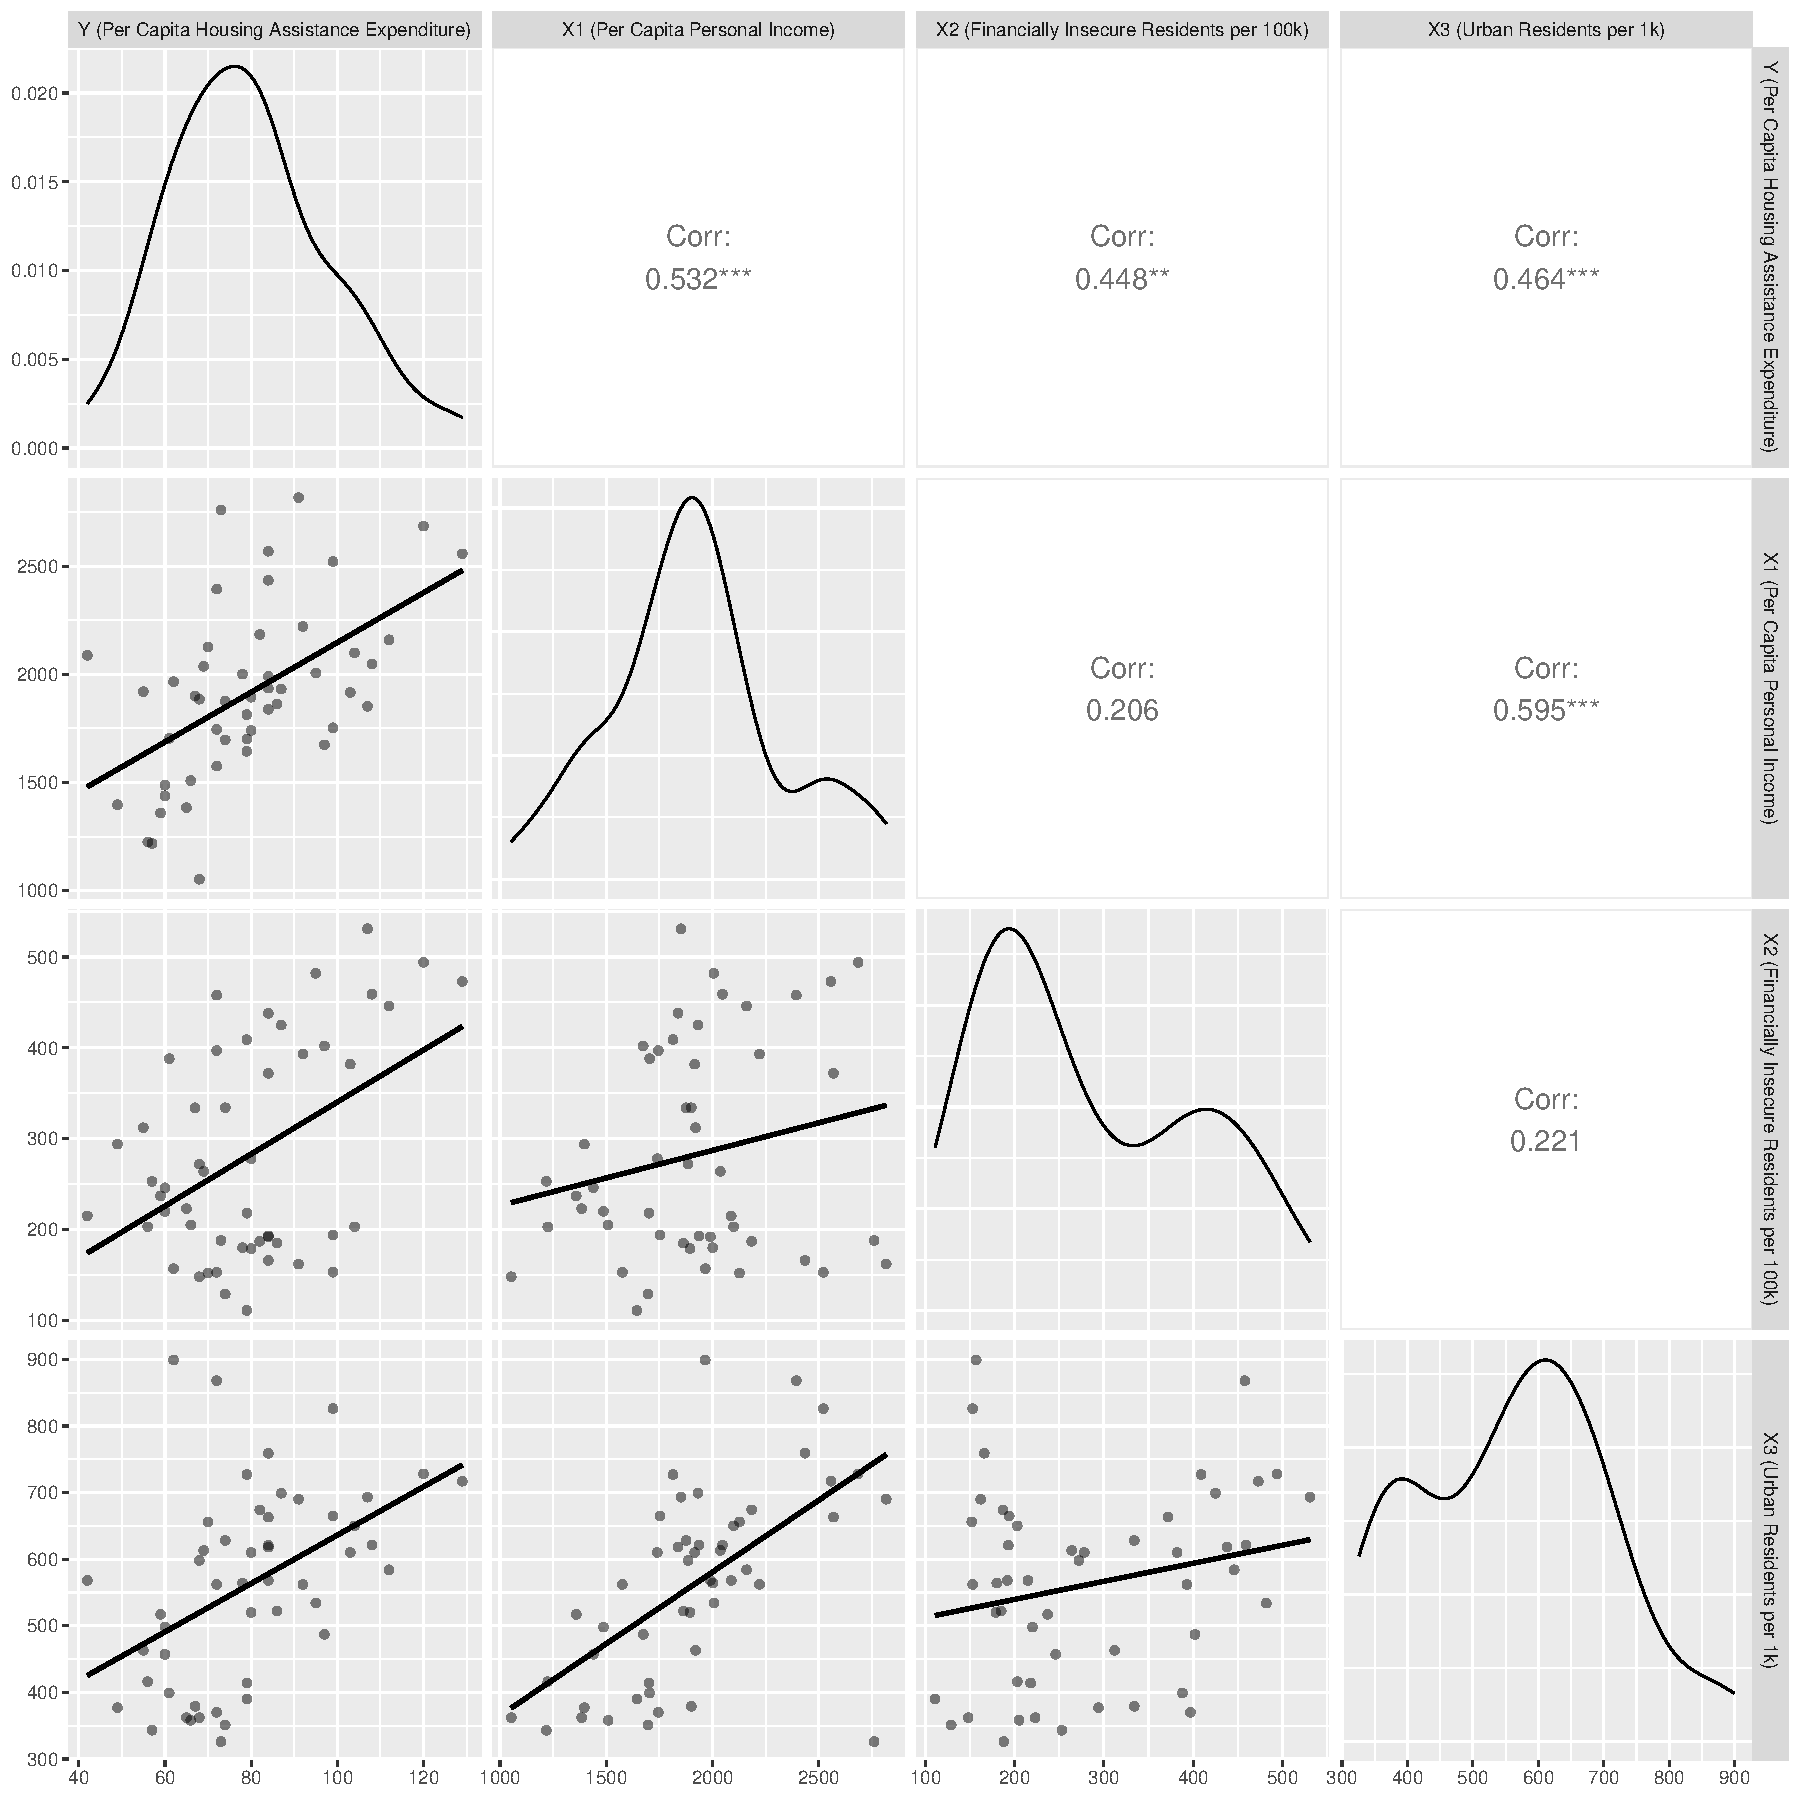
\includegraphics[width=0.8\textwidth]{graph2-1.pdf}
	\end{center}
	\vspace{.5cm}

	\textbf{Explanation}
	The figure was generated using the GGplot2 and GGaly (an extension of GGplot) libraries.
	
	The above figure (graph2-1.pdf) shows the pairwise scatterplots, density/distribution plots and correlation coefficients among Y, X1, X2 and X3. All the relationships appear to be positive, some more strongly than others. Per capita housing assistance expenditure (Y) appears to be moderately positively correlated with all three predictors: personal income X1 ($r \approx 0.53$), financially insecure residents X2 ($r \approx 0.45$) and urban residents X3 ($r \approx 0.46$). X1 and X3 appear to be fairly strongly correlated ($r \approx 0.60$), implying wealthier states might be more urban. X2 appears to be only weakly correlated with X1 ($r \approx 0.21$) and X3 ($r \approx 0.22$), as both graphs have a wide range of values and do not follow their lines of best fit (large residuals).
	\vspace{1cm}

	\item

	Please plot the relationship between \emph{*Y*} and \emph{*Region*}? On average, which region has the highest per capita expenditure on housing assistance?

	\vspace{1cm}

	\textbf{Code}
	\lstinputlisting[language=R, firstline=118, lastline=136]{PS01_answersEZ.R}
	\vspace{10cm}	
	\textbf{Generated Graph}

	\begin{center}
		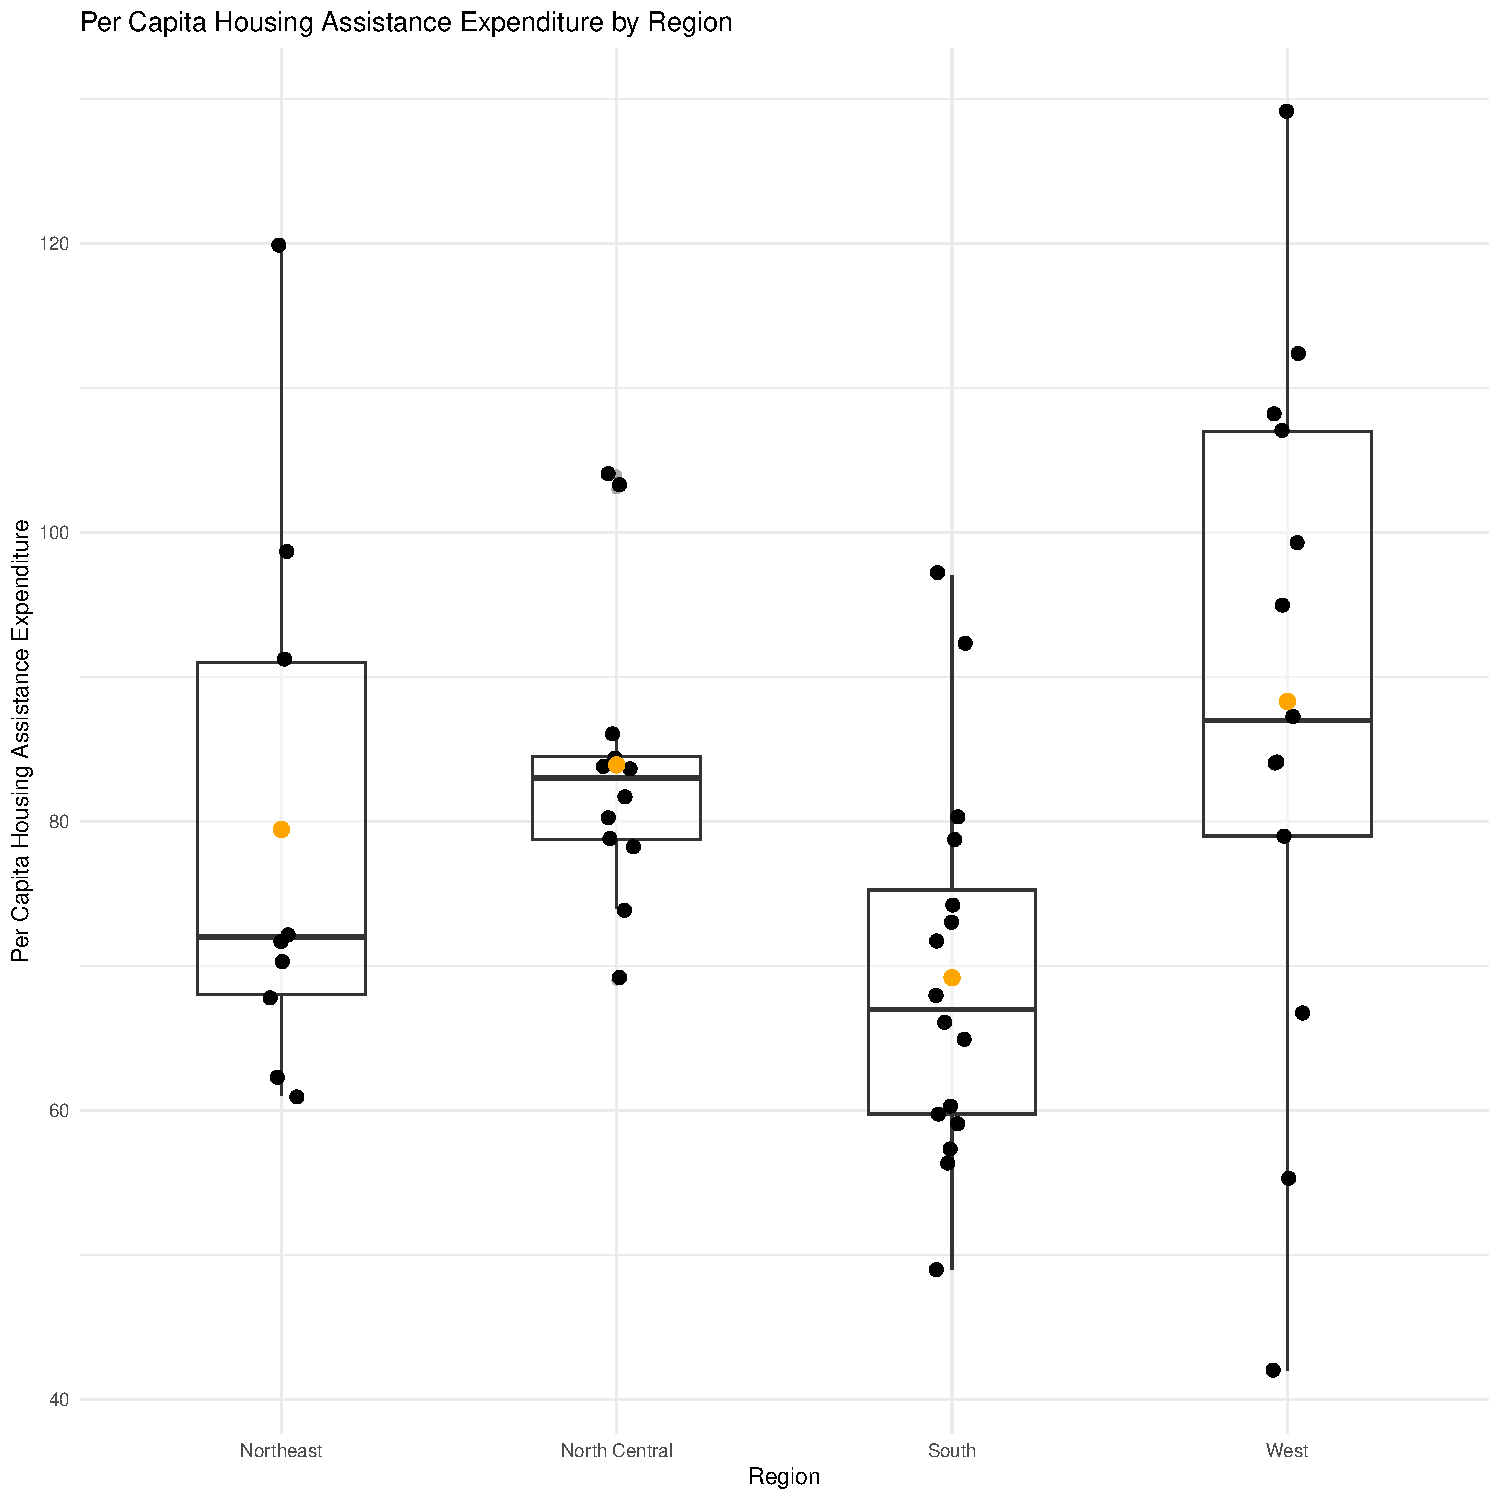
\includegraphics[width=0.8\textwidth]{graph2-2.pdf}
	\end{center}
	\vspace{.5cm}
	\textbf{Output}
	\begin{verbatim}
		Means by region:
		Northeast = 79.44
		North Central = 83.92
		South = 69.19
		West = 88.31 
	\end{verbatim}
	\textbf{Explanation}
		The boxplot of Y (per capita expenditure on shelters/housing) by Region (graph2-2.pdf, the orange dot marking each region's mean) shows that the West has the highest average per capita expenditure on housing assistance, at about 88.31. It is followed by the North Central region (about 83.92), the Northeast (about 79.44) and the South (about 69.19), which has the lowest average. The West also has the widest deviation, ranging from very low spending (Wyoming, 42) to the highest in the data (California, 129).
	\vspace{1cm}

	\item
	Please plot the relationship between \emph{Y} and \emph{X1}? Describe this graph and the relationship. Reproduce the above graph including one more variable \emph{Region} and display different regions with different types of symbols and colors.

	\vspace{1cm}

	\textbf{Code for First Graph (the relationship between Y and X1)}
	\lstinputlisting[language=R, firstline=140, lastline=151]{PS01_answersEZ.R}
	\vspace{11cm}

	\textbf{Generated Graph}
	\begin{center}
		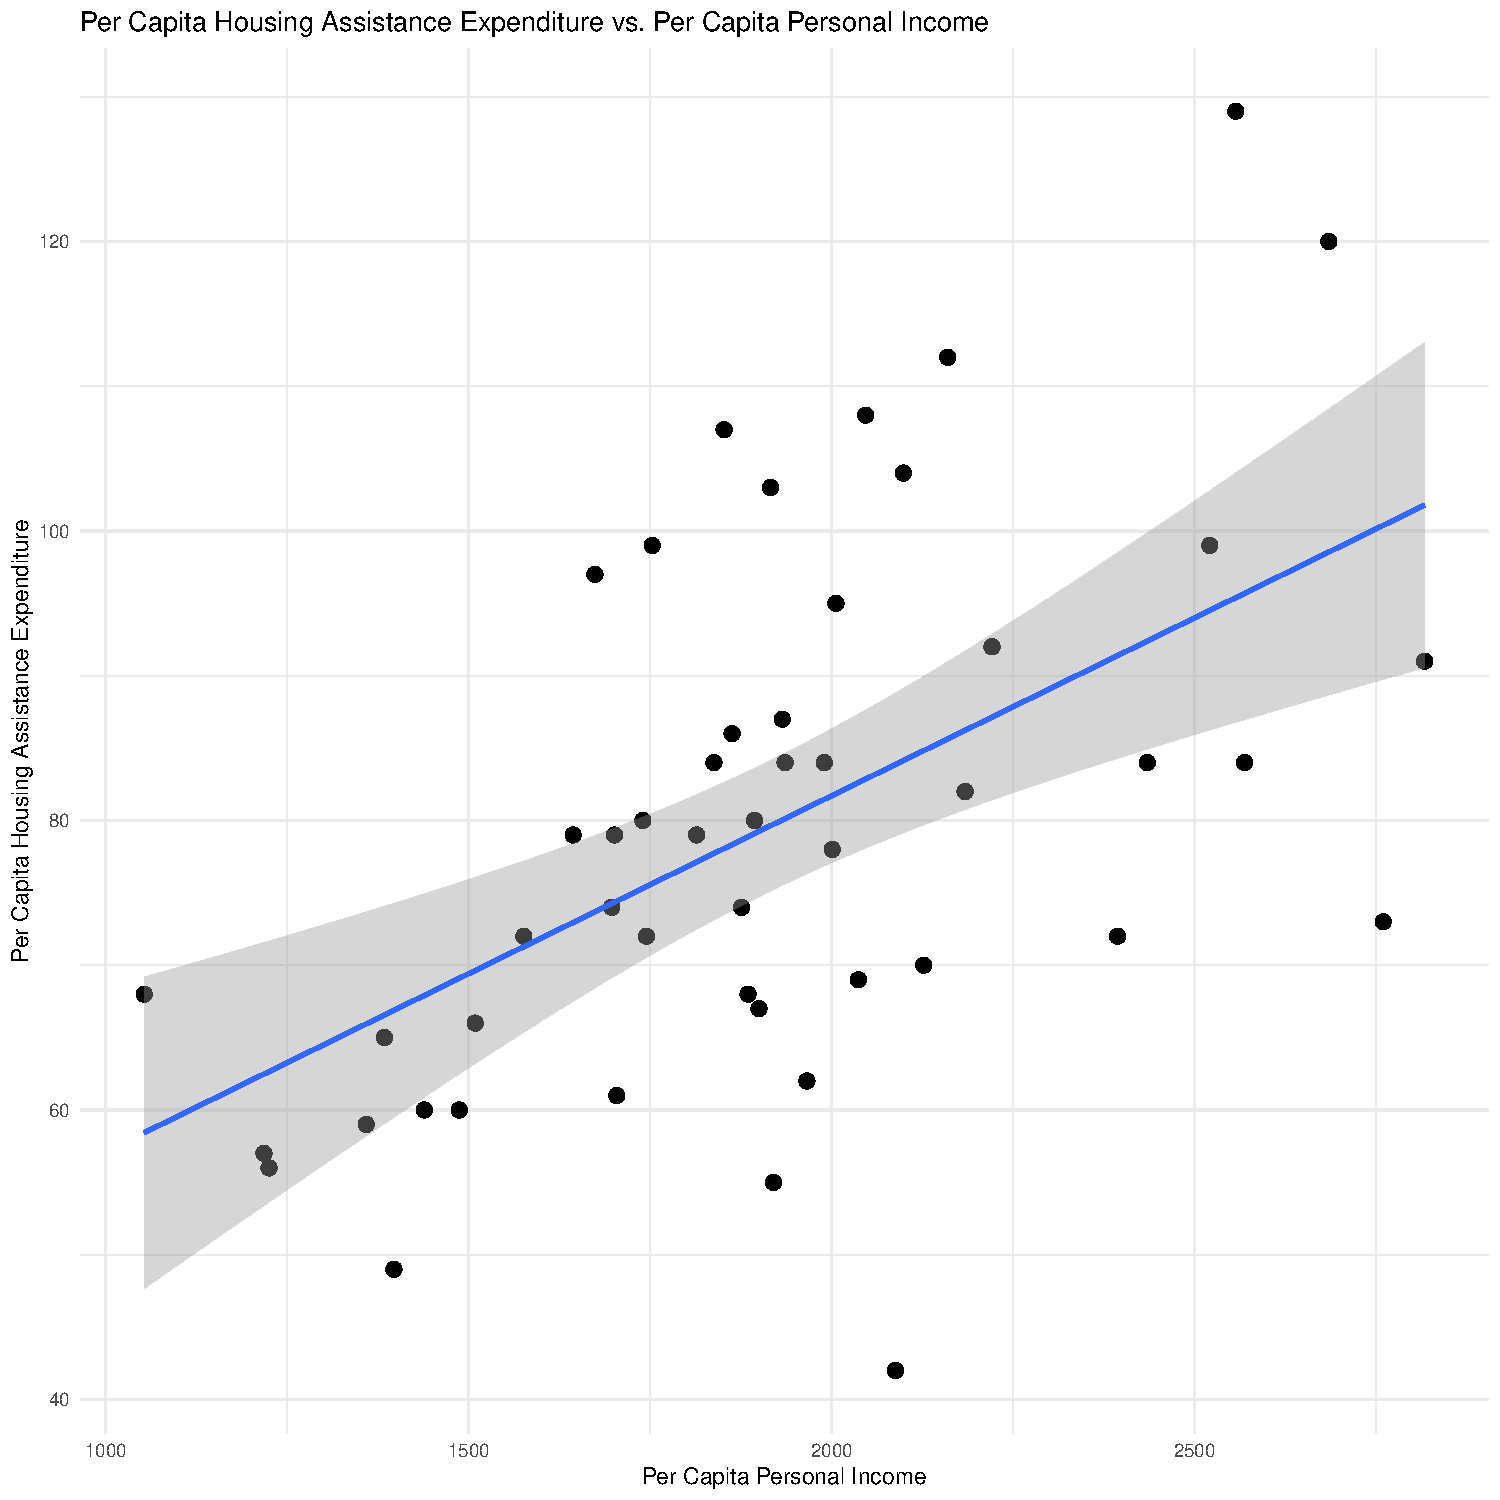
\includegraphics[width=0.8\textwidth]{graph2-3-1.pdf}
	\end{center}
	\vspace{.5cm}
	\textbf{Explanation}
		The scatterplot of Y against X1 (graph2-3-1.pdf) appears to have a positive, roughly linear relationship. This implies that states with higher per capita income tend to spend more per capita on housing assistance. The correlation is moderate and the points are widely scattered around the line, so income appears to explain only part of the variation in spending.
	\vspace{1cm}

	\textbf{Code for Second Graph (include region)}
	\lstinputlisting[language=R, firstline=155, lastline=173]{PS01_answersEZ.R}
	\vspace{.5cm}

	\textbf{Generated Graph}
	\begin{center}
		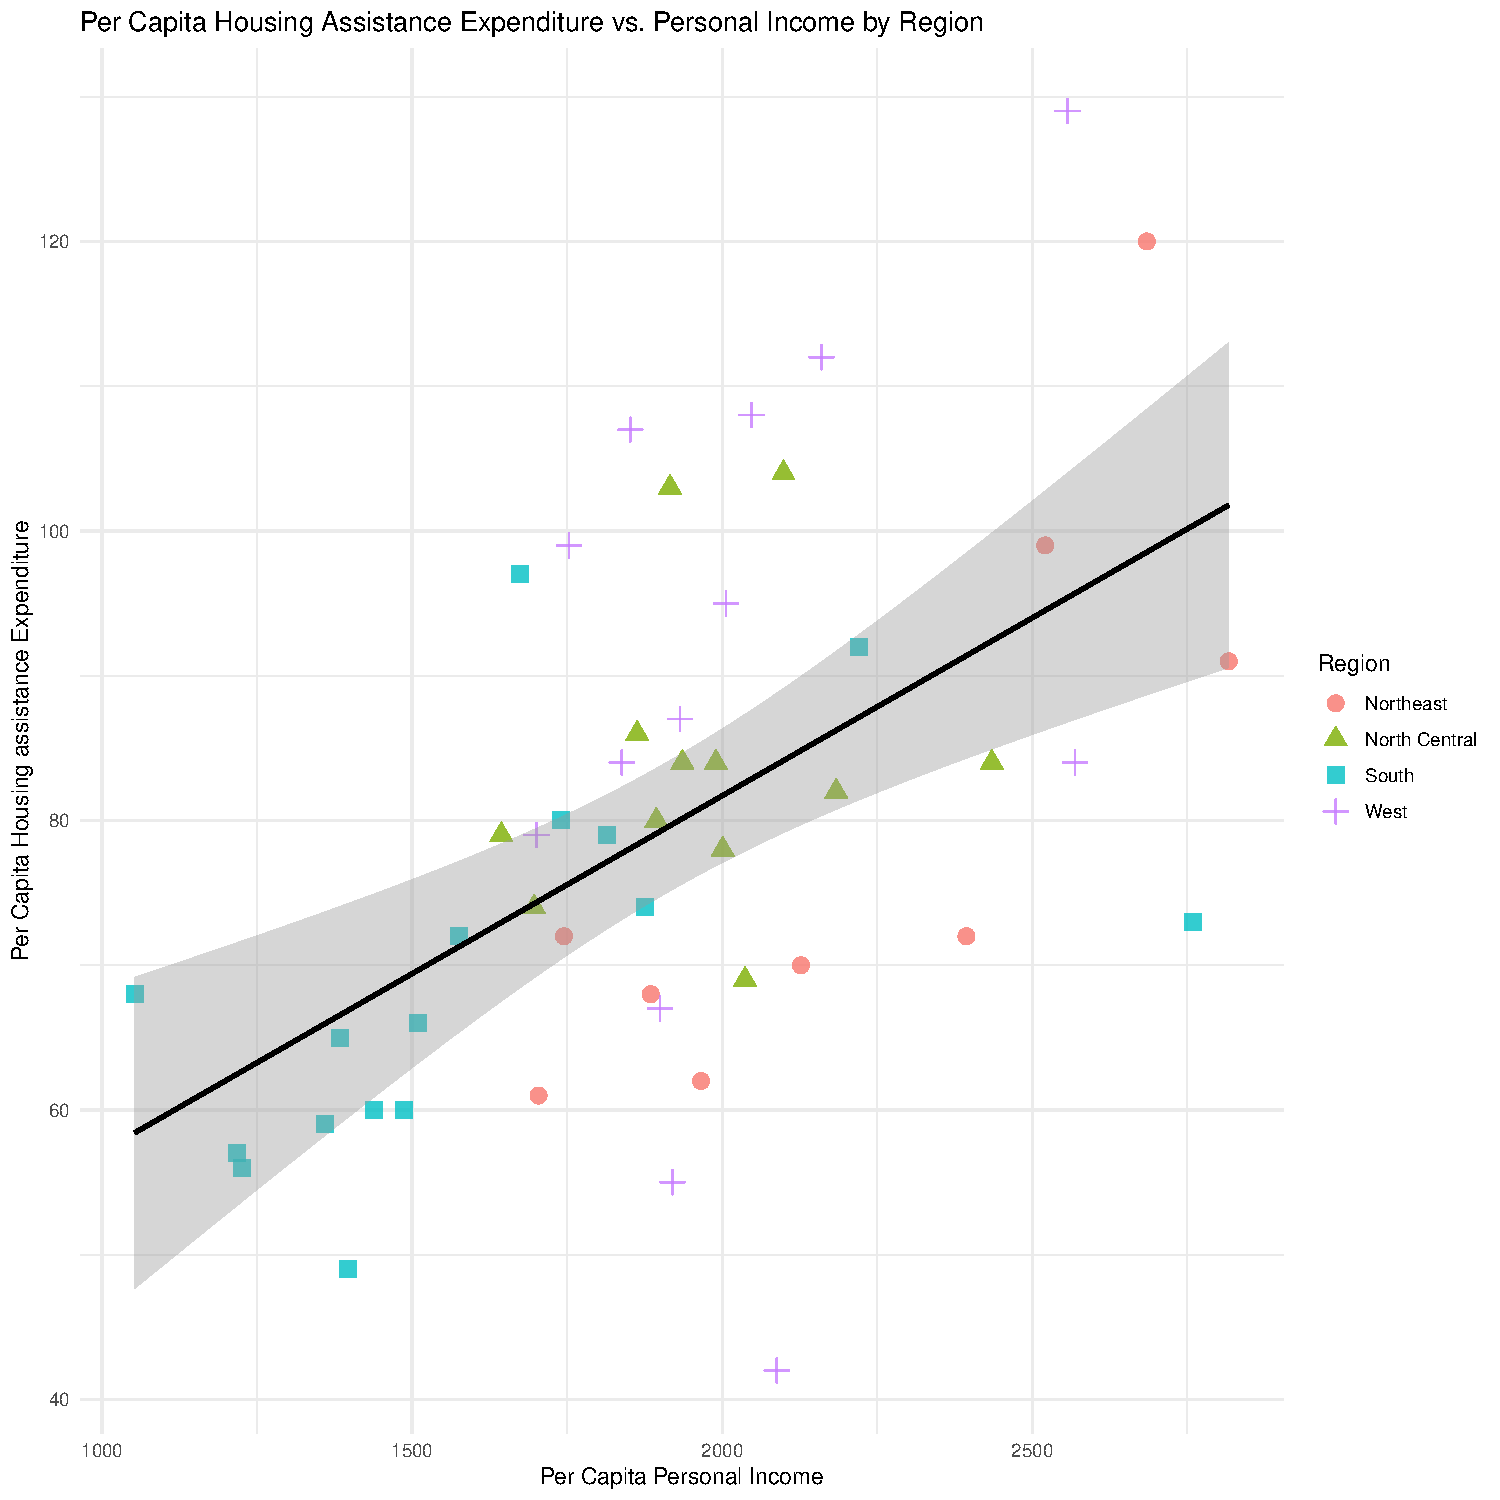
\includegraphics[width=0.8\textwidth]{graph2-3-2.pdf}
	\end{center}
	\vspace{.5cm}
	\textbf{Explanation}
The second graph (graph2-3-2.pdf) adds Region, with each region shown using its own color and symbol. The regions cluster in different parts of the plot. Southern states sit mostly in the lower left (low income, low spending), while Northeastern states sit toward the upper right, (higher income, higher spending. West and North Central states fall in between, although several Western states appear to spend a lot relative to their income. The positive relationship holds within every region. However, the degree varies by region. This suggests that part of the overall positive relationship reflects differences between regions rather than a uniform effect.
\end{itemize}

\end{document}